 %!TEX root = demo.tex
 \section{Data Cleaning API}
Designing declarative specifications for data cleaning has been studied before, most notably by the AJAX project \cite{DBLP:conf/vldb/GalhardasFSSS01}.
The operator specifications in the AJAX project were mainly aimed data integration tasks where the entire dataset is cleaned.
However, recent data cleaning frameworks avoid cleaning of entire datasets either through the use of sample-based result estimation or Machine Learning.
Inspired by that work, we design a new specification API that also incorporates these recent results.

\subsection{Operators}

\vspace{0.5em}

\noindent \textsf{SimilarityJoin(R,S,$\phi$, $t$)}: For a given relations $R(a_1,...,a_l)$ and $S(b_1,...,b_k)$, a similarity function $\phi$, and a threshold $t$, the similarity join of R and S is defined by:
\[
\{ (r,s) \in R \times S \text{ s.t } \phi (r,s) \ge t \}
\]

\vspace{0.5em}


\noindent \textsf{Filter(R, $\rho$)}: For a given relation $R(a_1,...,a_l)$ and a boolean condition $\rho$, return $R' \subseteq R$ that satisfies $\rho$.

\vspace{0.5em}

\noindent \textsf{Extract(R, a, $\epsilon$)} For a given relation $R(a_1,...,a_l)$, a attribute $a$, and an extraction function $\epsilon$, apply $\epsilon$ to every $R(a)$ returning $\epsilon(R(a)) = (v_1,...,v_k)$. The result relation is:
\[
R(a_1,...,a_l,\epsilon(R(a)))
\]

We can make the use of these operators clear based on an example from
our demonstration scenario.
\begin{example}[Social Media Analysis]
To clean \textsf{Comment}, we will first apply \textsf{Extract} to the \textsf{tags}
attributes and create additional columns for all the tags.
Then, we could apply a self \textsf{SimilarityJoin} on the projection of only the tag columns 
to group all of the similar tags.
Finally, we apply \textsf{Filter} to \textsf{SimilarityJoin} relation to remove pairs that
are not true matches.
\end{example}

\subsection{Learning Parameters From Example}
The magic in using the operators described above is setting the parameter functions $\phi$, $\rho$, and $\epsilon$.
In simple cases, it might be easy to use domain knowledge to program these functions. 
For example, if \textsf{tags} is consistently delimited by commas then it is clear how to specify $\epsilon$.
In more complex cases, it might be easier to specify a sample of dirty and clean data instead of the function.

In our current implementation of \projx, we pose this learning problem as classification problems.
In general, these parameter functions can be quite complex and this is a simplification of the learning problem.
The choice of classifier and featurization is upto the user. We currently support Support Vector Machines and Decision Trees with a featurization library that includes common text processing features.

\vspace{0.5em}

\noindent \textsf{SimilarityJoin(R,S,$\mathcal{T}^+$, $\mathcal{T}^-$)}: Given a set of positive training examples $\mathcal{T}^+$ (i.e, $(r,s)$ that are ``similar") and
negative training examples $\mathcal{T}^-$ (i.e, $(r,s)$ that are  ``not similar"), we learn a classifier that predicts whether two records are similar or not. 

\vspace{0.5em}


\noindent \textsf{Filter(R, $\mathcal{T}^+$, $\mathcal{T}^-$)}: Given a set of positive training examples $\mathcal{T}^+$ (i.e, $r$ that satisfy the condition) and
negative training examples $\mathcal{T}^-$ (i.e, r that do not satisfy the condition), we learn a classifier that predicts whether a record satisfies the condition. 

\vspace{0.5em}

\noindent \textsf{Extract(R, a, $\mathcal{T}$)} We restrict the learned problem setting to delimited extraction. Given a set of training examples $R(a)$ and the output $v_1,v_2,...,v_k$, we learn a classifier to predict which characters in $R(a)$ are delimiters based on the tokens in the string.

\subsection{Selecting Examples}
An important question is how to selecting these training examples. 
We provide two techniques to select records to generate these examples.

\noindent\textbf{Uniform Sampling: } Uniform random sampling is an important primitive in sample-and-clean systems. Given a relation $R$, we take a uniform random sample of ratio $m\in[0,1]$ which means that every record has a probability $m$ of being in the sample. We provide both hash-modulo based and coin-flip based variants for sampling.

\noindent\textbf{Active Learning: } In Active Learning, we select the most informative next record to add to our training example set. Given a set of training examples $\mathcal{T}$ and a learned classifier, we select the next record using a technique called uncertainty sampling. Intuitively, when the classifiers learned are confident in their predictions (e.g, the points are far from the margin in an SVM) then providing that example in uninformative, however, when the uncertainty is higher those are the examples we need to provide. A typical Active Learning workflow starts with a small uniform sample.

\subsection{Crowd Microtasks}
After we select the training examples, the next step is to actually clean those records.
We expose an interface to collect that data through crowd microtasks.
We decompose high-level data cleaning operations into three basic crowd tasks: Pair Comparison, Condition Checking, and Data Entry.
These tasks are served by a browser interface that is compatible with both Amazon Mechnical Turk and a stand-alone webserver.

\noindent\textbf{Pair Comparison: } Given a pair of records, a crowd worker indicates if they are the same or are different. In Figure \ref{fig:pair},
we illustrate an example pair comparison task.

\begin{figure}[ht!]
\centering
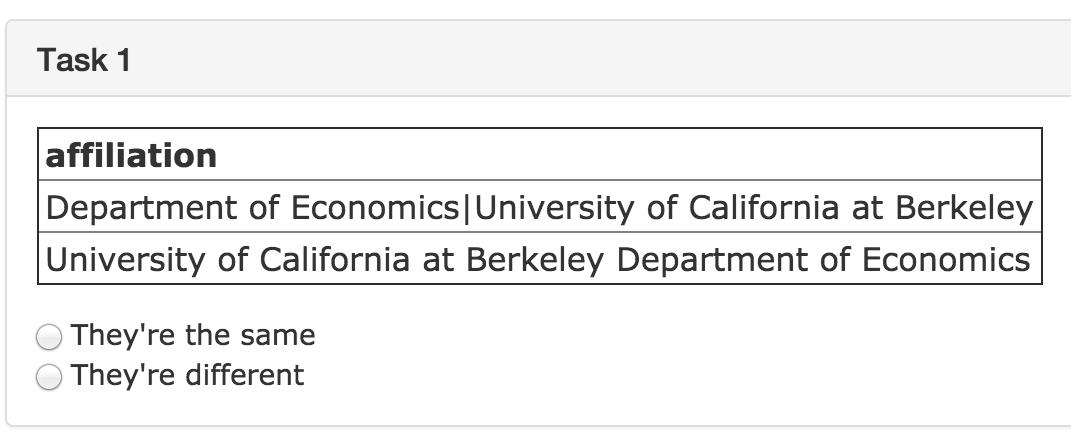
\includegraphics[scale=0.25]{figs/pair.png}
\caption{ \label{fig:pair}}\vspace{-.5em}
\end{figure}

\noindent\textbf{Condition Checking: } Given a single record, a crowd worker indicates if it satisfies some condition. In Figure \ref{fig:condition},
we illustrate an example condition checking task.
\begin{figure}[ht!]
\centering
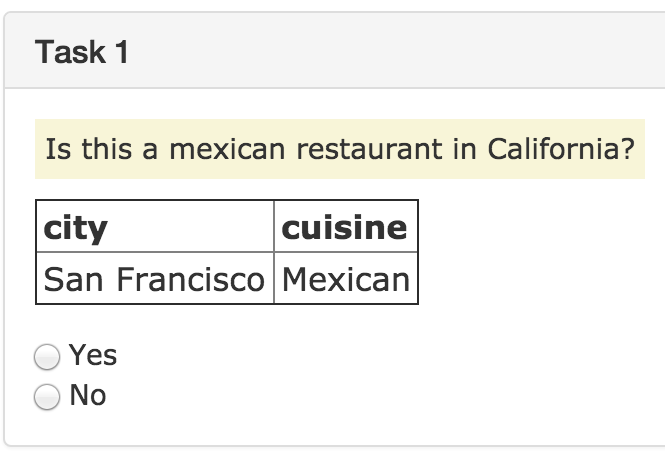
\includegraphics[scale=0.25]{figs/condition.png}
\caption{ \label{fig:condition}}\vspace{-.5em}
\end{figure}

\noindent\textbf{Data Entry: } Given a single record and a missing attribute, a crowd worker enters the missing value. In Figure \ref{fig:entry},
we illustrate an example data entry task.

\begin{figure}[ht!]
\centering
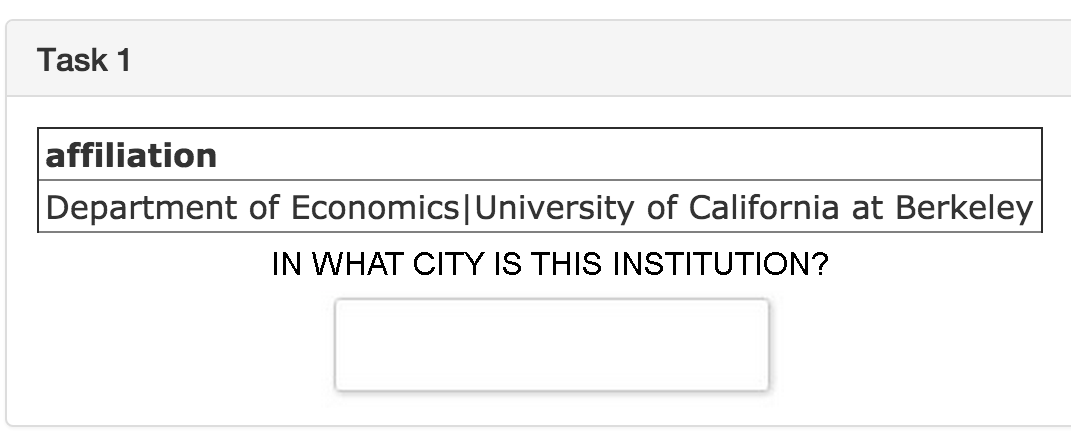
\includegraphics[scale=0.25]{figs/entry.png}
\caption{ \label{fig:entry}}\vspace{-.5em}
\end{figure}




